\section{Reducción de dimensionalidad}

\subsection{Introducción}
Como se mencionó previamente este ejercicio consistió en reducir la dimensión
del espacio original de los datos, la cual era de 850 componentes, en un
espacio de 9 componentes. El objetivo fue el de capturar las componentes que
mas explican la variabilidad de los datos en un espacio de dimensión menor.
Para esto se utilizaron redes neuronales entrenadas con los algoritmos de
\textit{Oja} y \textit{Sanger}. Al final del entrenamiento estos métodos
terminan habiendo modificado los pesos de la red de forma tal que su función
asociada sea la de proyectar el vector del espacio original en el subespacio de
las primeras componentes principales.

\subsection{Desarrollo}
La red neuronal que se utilizó para reducir dimensionalidad fue un perceptron
simple con función de activación lineal. Esta red contó con 850 neuronas de
entrada y 9 neuronas de salida. Esta topología fue pensada para poder
clasificar de forma no supervisada los documentos en 9 tipos de categorías.

Las reglas de actualización de pesos que se utilizaron fueron los de \textit{Oja} y
 \textit{Sanger} que son las que se describen a continuación

\begin{center}
	\begin{tabular}{rccc}
		\emph{Oja}: & $\Delta W_{ij}$ & = & $\eta \cdot y_{j} \cdot (x_{i} - \displaystyle\sum_{k = 0}^{m-1} W_{ki} \cdot y_{k} )$ \\
		\emph{Sanger}: & $\Delta W_{ij}$ & = & $\eta \cdot y_{j} \cdot (x_{i} - \displaystyle\sum_{k = 0}^{j} W_{ki} \cdot y_{k} )$ \\
	\end{tabular}
\end{center}

 % cuyos pseudocodigos se presentan a continuacion:
% %%%%%%%%%%%%%%%%%%%%%% PONER PSEUDO DE OJA Y SANGER %%%%%%%%%%%%%%%%%%%%%%%%%%%%%

Se decidió separar el conjunto de datos en entrenamiento y testing con una
proporción de 90\% y 10\% respectivamente. Los hiper-parámetros utilizados para
el entrenamiento de la red fueron $\eta = 0.0001$ y 1000 épocas. La razón por
la que se decidió utilizar un coeficiente de entrenamiento de una magnitud tan
pequeña fue que los datos de entrada no estaban normalizados, logrando que
ocurran errores de overflow.

\subsection{Resultados}
Para una visualización mas clara de los datos se decidieron realizar tres
gráficos diferentes en el que cada uno muestra de a tres componentes
principales. Se decidieron graficar los datos de testing con un marcador con
forma de triangulo para diferenciarlo de los círculos que representan los datos
de entrenamiento. Los resultados obtenidos se presentan a continuación:


\begin{figure}[H]
  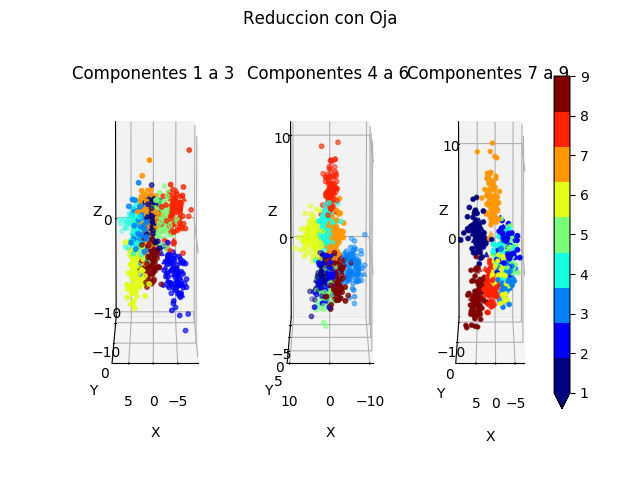
\includegraphics[width=0.9\textwidth]{imagenes/componentes_oja_1.png}
  \caption{Vista desde arriba con Oja}
\end{figure}

\begin{figure}[H]
  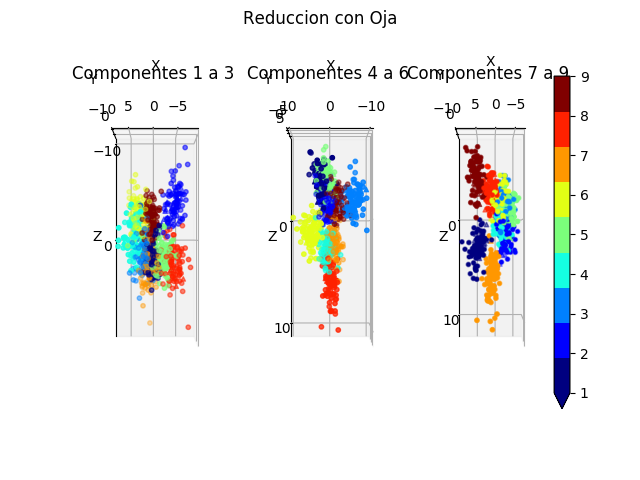
\includegraphics[width=0.9\textwidth]{imagenes/componentes_oja_2.png}
  \caption{Vista desde abajo con Oja}
\end{figure}

\begin{figure}[H]
  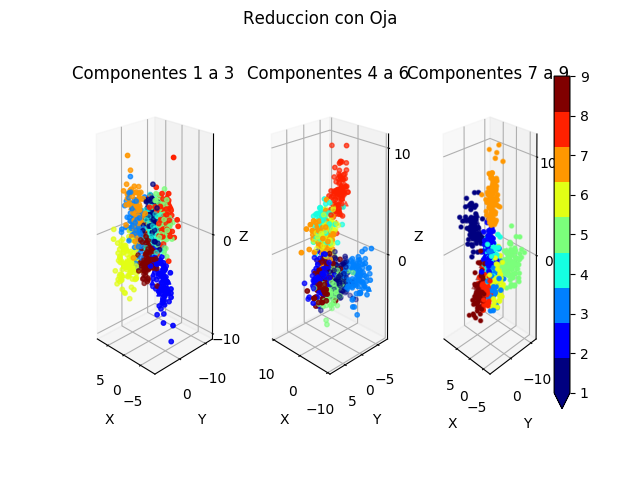
\includegraphics[width=0.9\textwidth]{imagenes/componentes_oja_3.png}
  \caption{Vista de costado con Oja}
\end{figure}

\begin{figure}[H]
  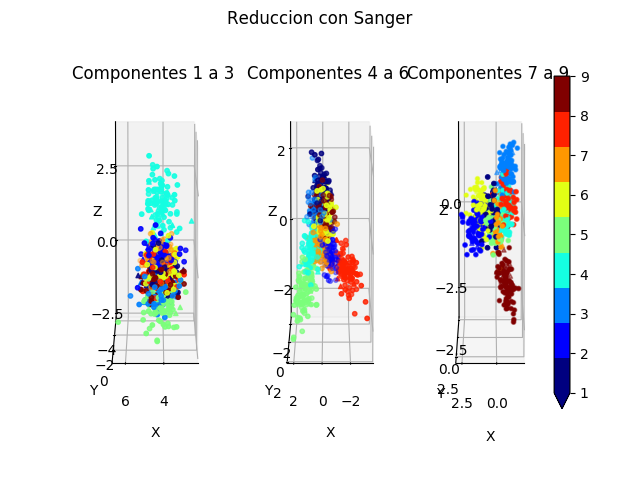
\includegraphics[width=0.9\textwidth]{imagenes/componentes_sanger_1.png}
  \caption{Vista desde arriba con Sanger}
\end{figure}

\begin{figure}[H]
  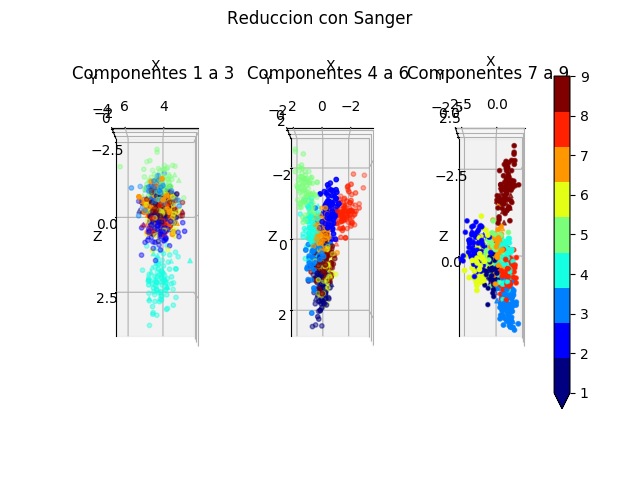
\includegraphics[width=0.9\textwidth]{imagenes/componentes_sanger_2.png}
  \caption{Vista desde abajo con Sanger}
\end{figure}

\begin{figure}[H]
  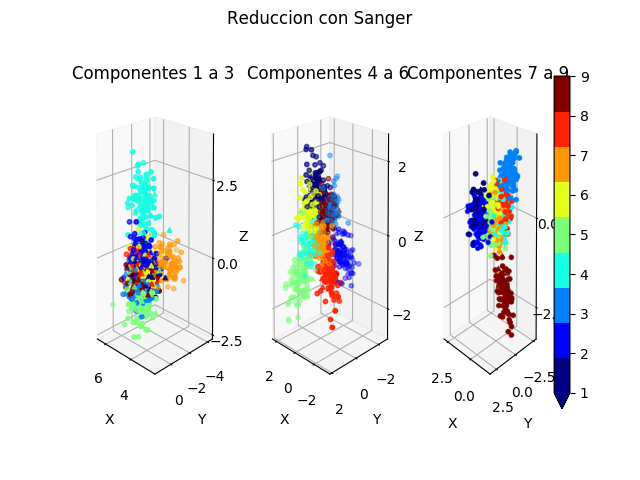
\includegraphics[width=0.9\textwidth]{imagenes/componentes_sanger_3.png}
  \caption{Vista de costado con Sanger}
\end{figure}

Se observó que los vectores generados por el algoritmo de Sanger son mas
descriptivos en comparación a los generados por Oja.  Es decir, que lograron
una mejor separación de los datos. Una posible justificación a este
razonamiento es que los pesos generados por el algoritmo de Sanger convergen
siempre al mismo vector, generando con ello siempre la misma proyección.

\clearpage

\subsection{Conclusión}
Como conclusión se pudo destacar que al tener los datos proyectados en las 9
componentes principales se pueden ver 9 clusters bien diferenciados
espacialmente.  Esto logra la posibilidad de clasificar fácilmente los
documentos en 9 categorías distintas mediante la aplicación de un clasificador
como por ejemplo un perceptron multicapa.  También se mejoraría los tiempos de
entrenamiento ya que luego de ser preprocesada la entrada, los datos tienen una
dimensión menor y por lo tanto la entrada del clasificador es mucho mas chica.

Estos modelos por si solos no sirven para clasificar, sino mas bien para darse
una idea de cuantas clases hay dentro de los datos de entrada. También sirven
para preprocesar la entrada que luego será ingresada en un clasificador,
conformando así un modelo de tipo híbrido.
\newpage
